\subsection{Optical Flow} 
El campo de movimiento de una imagen es el movimiento real del objeto en el espacio proyectado sobre el plano de la imagen. El Optical Flow (flujo óptico) se define como el flujo de la intensidad en escala de grises en el plano de la imagen, a medida que evoluciona en el tiempo. También se puede interpretar el flujo de la imagen como el movimiento aparente de esta basado en la percepción visual, teniendo dimensión de velocidad $\vec{V}= (V_x \ , \ V_y)$. Si el Optical Flow se determina de dos imágenes consecutivas, aparece un vector de desplazamiento $\vec{d}$ de las cualidades elegidas, entre el cuadro n y el n+1.
\begin{figure}[H]
		\centering
		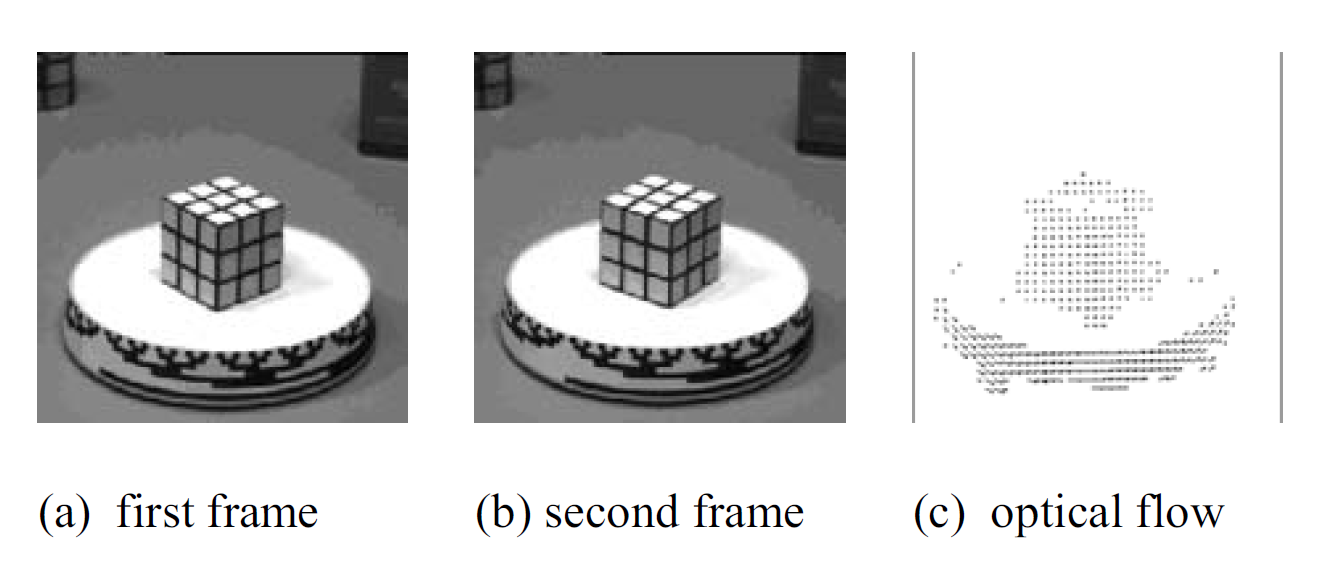
\includegraphics[width=0.5\textwidth]{Imagenes/opticalflowrubick.png}
		\caption{Cubo de rubik rotando en una mesa.}
		\label{fig:opticalflow1}
\end{figure}
Para la implementación del algoritmo existen varios caminos, como lo es, por ejemplo, el basado en calculo de gradientes de la imagen total. Existe otro que utiliza solo ciertos puntos que se determinan constantes de la imagen. El el presente se emplea el método piramidal de Lucas-Kanade.

\subsubsection{Lucas-Kanade} 
Este algoritmo consta del uso de información obtenida a partir de la intensidad del gradiente espacial para buscar la posición que mejor se acomoda a una imagen en movimiento \cite{ref:lucas-kanade} \cite{ref:lucas-kanade2}. Algunas de las hipótesis que postula Lucas-Kanade son:
\begin{itemize}
\item Los movimientos entre cuadros consecutivos son pequeños. Tan pequeños como un pixel.
\item La intensidad de los objeto se mantiene constante cuadro a cuadro.
\end{itemize} 
Este algoritmo se basa en el principio de ``divide y conquistarás'' al realizar la tarea de detectar movimiento en toda la imagen en problemas más sencillos. El proceso consta de dividir la pantalla en un árbol cuaternario. Esto lo hace debido a que se requiere que las hipótesis de Lucas-Kanade deben cumplirse, se toma una pequeña parte de la imagen, del menor tamaño posible, donde tienden a cumplirse las condiciones necesarias del algoritmo. De allí se calcula recursivamente cada partición hasta el primer nivel.
\begin{figure}[H]
		\centering
		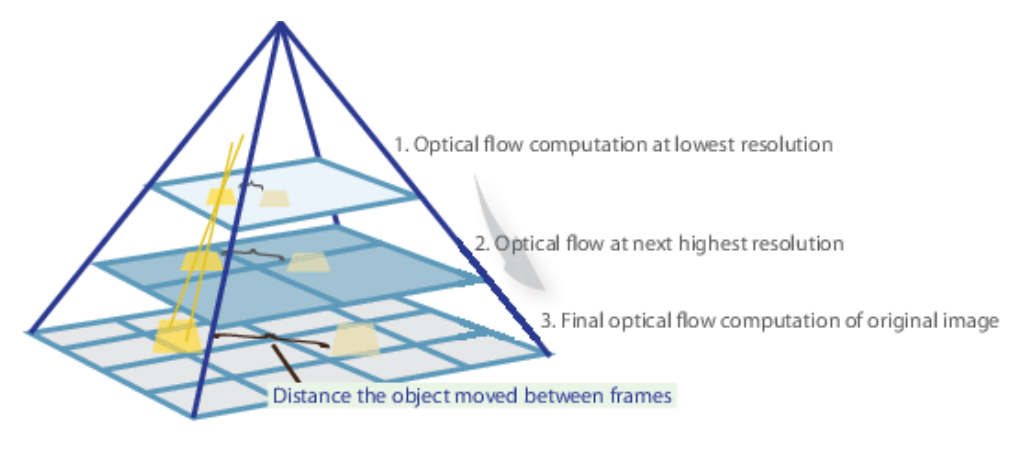
\includegraphics[width=0.5\textwidth]{Imagenes/op.png}
		\caption{Cálculo del Optical Flow.}
		\label{fig:opticalflow1}
\end{figure}
\subsection{Shi-Tomasi}

Por su parte, el algoritmo de Shi-Tomasi se basa en el algoritmo de Harris para la detección de bordes. El funcionamiento del algoritmo se basa en asignarle un valor a cada pixel del bitmap recibido, y si el valor del pixel es mayor a cierto límite se determina que este corresponde a una esquina. El valor asignado al pixel se obtiene utilizando dos autovalores de una matriz Z. Una función recibe estos autovalores, para poder manipularlos y devolver el valor.
La diferenciación entre el algoritmo de Harris y el de Shi-Tomasi, es que mientras Harris utiliza la función mencionada previamente, Shi-Tomasi decide utilizar únicamente los autovalores \cite{ref:shi-tomasi}.
\\ Los valores de cada pixel se determinan de la siguiente manera:

\begin{figure}[H]
\begin{align}
R= det(Z) - k (trace Z )^2 \\
det(Z)= \lambda_1 \cdot \lambda_2 \\
trace Z = \lambda_1 + \lambda_2
\end{align}
\label{eq:harris}
\caption{Valor de pixel para algoritmo de Harris}
\end{figure}

\begin{figure}[H]
\begin{align}
R= min(\lambda_1 , \lambda_2)
\end{align}
\label{eq:shitom}
\caption{Valor de pixel para algoritmo de Shi-Tomasi}
\end{figure}

\begin{figure}[H]
\centering
	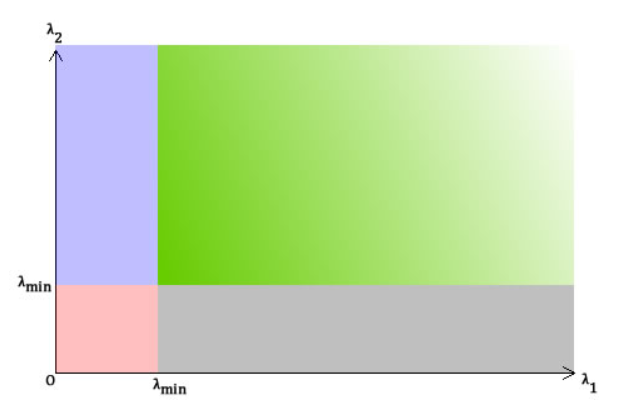
\includegraphics[width=0.4\textwidth]{Imagenes/shitom.png}
	\caption{Detección de bordes Shi-Tomasi.}
	\label{fig:shitom}

\end{figure}
\begin{itemize}
\item La zona verde corresponde a ambos $\lambda_1 \ y \ \lambda_2 $ mayores al valor límite, por lo que estos píxeles son tomados como esquina.
\item La zona azul y gris corresponden a que uno de los autovalores es menor al límite.
\item La zona roja corresponden a ambos autovalores menores al mínimo.
\end{itemize}
\subsection{Filtro de Kalman}
El filtro de Kalman es un filtro recursivo que busca estimar el estado de un sistema dinámico lineal discretizado de dimensión $n$ mediante una serie mediciones con ruido a partir de la descripción del modelo físico que rige las variables del vector de estado\cite{ref:kalman1}, \cite{ref:kalman2}.

\subsubsection{Planteo del problema}
Dado un proceso estocástico lineal en tiempo discreto definido por

\begin{equation}
x_k = Ax_{k-1} + w_{k-1} \footnote{Se omitió por simplicidad la función de control.}
\end{equation}

donde $x_k \in \mathcal{R}^{N}$ y siendo una medición en tiempo $k$ definida por

\begin{equation}
z_k = Hx_k + v_k
\end{equation}

con $z_k \in \mathcal{R}^m$, donde $w_k$ y $v_k$ son variables aleatorias que representan el ruido del proceso y de observación respectivamente, las cuales se asumen que son independientes entre sí y con distribuciones de probabilidad normales multivariadas definidas como

\[ p(w) \sim N(0, Q) \]

\[ p(v) \sim N(0, R) \]

donde $Q$ y $R$ son las matrices de covarianza del ruido del proceso y ruido de medición respectivamente, las cuales se asumen constantes; donde la matriz de transición de estados $A$ de dimensión $n\times n$ \textemdash siendo $n$ la dimensión de estados dinámicos del modelo\textemdash \ define la relación entre estados del paso $k-1$ al paso $k$ sin contar el ruido del proceso; donde la matriz de transición de observación $H$ de dimensión $m\times n$ \textemdash siendo $m$ la dimensión del vector de medición\textemdash \  fija la relación entre el espacio de  los observables medidos y el espacio de las variables del vector de estados, sin contar el ruido de medición; y finalmente donde el estado del filtro puede representarse como $\hat{x}_{k|k}$ y $P_{k|k}$, siendo estos el estimador del vector de estados a posteriori dadas las mediciones hasta un tiempo $k$, y el estimador de la matriz de covariaza a posteriori dadas las mediciones hasta un tiempo $k$ respectivamente. Se puede definir la operación del filtro de Kalman separando a esta en dos fases: la predicción, y la corrección.

\subsubsection{Ecuaciones de predicción}

\begin{equation}
\hat{x}_{k|k-1} = A\hat{x}_{k-1|k-1}
\end{equation}
\begin{equation}
P_{k|k-1} = AP_{k-1|k-1}A^T + Q
\end{equation}

\subsubsection{Ecuaciones de observación}

\begin{equation}
\hat{x}_{k|k} = \hat{x}_{k|k-1} + K_k y_k
\end{equation}
\begin{equation}
P_{k|k} = (\mathbb{I}-K_kH)P_{k|k-1}
\end{equation}

donde,

\begin{equation}
y_k = z_k - H\hat{x}_{k|k-1}
\end{equation}
\begin{equation}
S_k = HP_{k|k-1}H^T + R_k
\end{equation}
\begin{equation}
K_k = P_{k|k-1}H^TS_k^{-1}
\end{equation}

\begin{figure}[H]
		\centering
		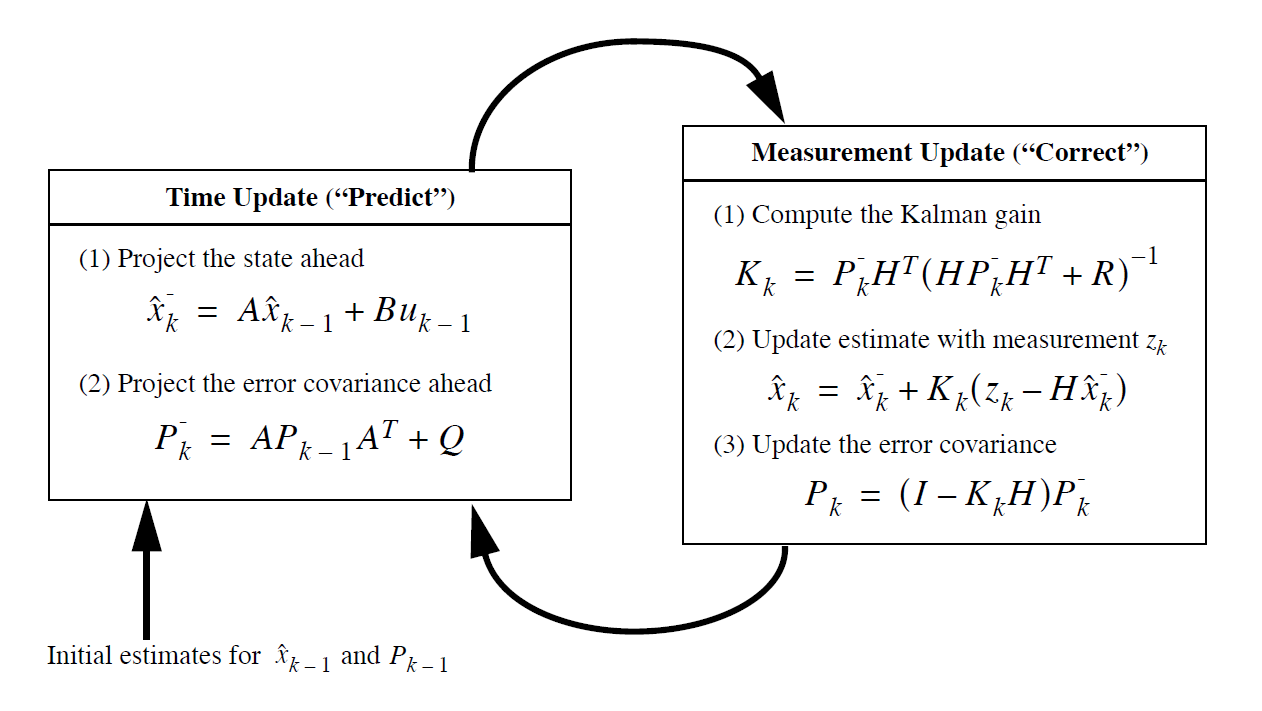
\includegraphics[width=0.5\textwidth]{Imagenes/kalman1.png}
		\caption{Funcionamiento completo del filtro Kalman simple \cite{ref:kalman2}.}
		\label{fig:kalman1}
\end{figure}




 En la Figura (\ref{fig:kalman-comp}) se puede observar el funcionamiento del algoritmo con un vector de estados dinámicos de dimensión dos compuesto por las coordenadas $(x,y)$ sobre el plano cartesiano. Realizando mediciones periódicamente, se comparan dos curvas. Por un lado, una senoidal con un ruido gaussiano montado sobre ella, simulando una serie de mediciones con ruido, y por el otro lado, la estimación obtenida a partir del filtro desarrollado.

\begin{figure}[H]
\centering
	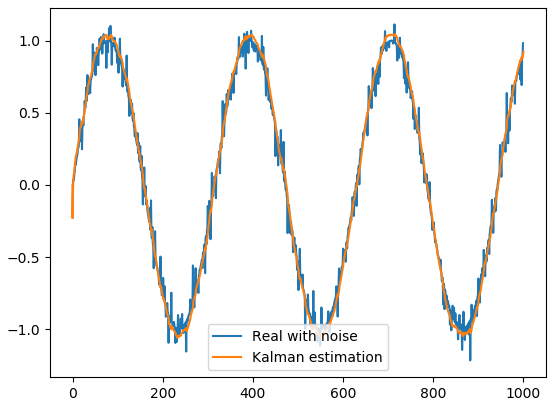
\includegraphics[width=0.4\textwidth]{Imagenes/Kalman_test_1.png}
	\caption{Seno con ruido comparada con estimación de Kalman.}
	\label{fig:kalman-comp}
\end{figure}

\subsection{Filtros de Correlación:}
\label{sec:corr}
El filtro de correlación o también conocido como ``Matched Filter'' \cite{ref:Corr} en inglés, se obtiene al calcular la correlación de una señal conocida, o ``kernel'', con una señal desconocida con el propósito de detectar este kernel en la última señal. Esto último es equivalente a convolucionar la señal desconocida con la inversión temporal del conjugado de la conocida. Este filtro es el óptimo lineal que maximiza la relación señal a ruido (SNR) en presencia de ruido aditivo.

Existen diversas maneras de calcular esta correlación, los dos métodos propuestos fueron:
\begin{itemize}
\item Cuadrados mínimos:
Se basa en el cálculo de cuadrados mínimos entre el kernel y la imagen mientras se realiza la convolución y corresponde a la siguiente ecuación
\begin{align}
R(x,y) = \frac{\Sigma_{x',y'} \left( T(x',y') - I(x+x',y+y') \right)^2}{\sqrt{\Sigma_{x',y'} T(x',y')^2  \cdot \Sigma_{x',y'}  I(x+x',y+y')^2}}
\end{align}
\item Estimación de la correlación:
Se calcula la correlación por definición del frame con respecto al kernel a medida que se desliza por la imagen, le corresponde la siguiente fórmula
\begin{align}
R(x,y) = \frac{\Sigma_{x',y'} \left( T(x',y') \cdot I(x+x',y+y') \right)}{\sqrt{\Sigma_{x',y'} T(x',y')^2  \cdot \Sigma_{x',y'}  I(x+x',y+y')^2}}
\end{align}
\end{itemize}
Donde R es la función de resultado, I la señal desconocida, y T el template o kernel.

A continuación se muestra una imagen y el resultado del cálculo de correlación utilizando la correlación por cuadrados mínimos y por correlación.

\begin{figure}[H]
\centering
	\begin{subfigure}{.4\textwidth}
		\centering
		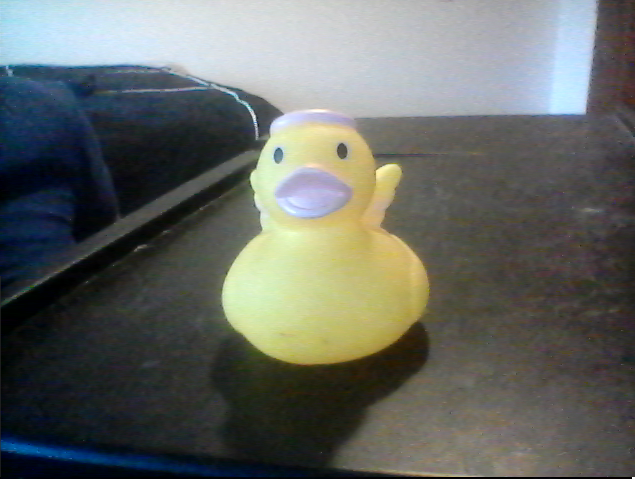
\includegraphics[width=0.8\textwidth]{Imagenes/Original.png}
		\caption{Imagen Fuente.}
		\label{fig:original}
	\end{subfigure}
	\begin{subfigure}{.4\textwidth}
		\centering
		
\includegraphics[width=0.8\textwidth]{Imagenes/Correlation.png}
		\caption{Correlación utilizando definición.}
		\label{fig:corr}
	\end{subfigure}
		\begin{subfigure}{.4\textwidth}
		\centering
		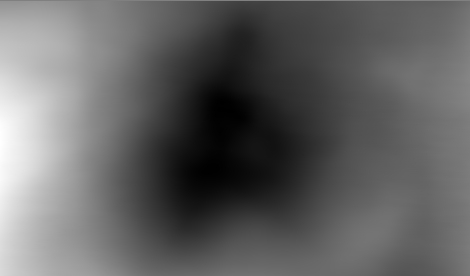
\includegraphics[width=0.8\textwidth]{Imagenes/SQDIFF.png}
		\caption{Correlación utilizando cuadrados mínimos.}
		\label{fig:sqdiff}
	\end{subfigure}
	\begin{subfigure}{.1\textwidth}
		\centering
		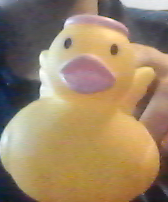
\includegraphics[width=1.2\textwidth]{Imagenes/kernel.png}
		\caption{Kernel.}
		\label{fig:kernel}
	\end{subfigure}
	\caption{Aplicación del algoritmo de correlación.}
	\label{fig:corrtest}
\end{figure}
Se puede apreciar como el punto más oscuro de la pantalla indica el punto de mayor correlación entre la imagen fuente y el kernel seleccionado para el algoritmo de cuadrados mínimos mientras que el mas claro indica la mayor correlación para el otro. 
\subsection{Filtros basados en distribución de probabilidad de Hue:}
Los filtros de color tradicionales usualmente se basan en la detección de un color especifico con la adición de una cierta tolerancia para poder incluir una gama de colores más amplia. Sin embargo dicha elección resulta ser demasiado restrictiva cuando aparecen sombras o cambios de iluminación. Es por eso que una alternativa más permisiva es la de utilizar mascaras que permitan el paso de ciertos colores según una función de masa de probabilidad dada. Dicha distribución se computa usando como semilla el objeto que deseamos seguir.
\begin{figure}[H]
\centering
	\begin{subfigure}{.1\textwidth}
		\centering
		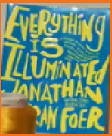
\includegraphics[width=1.2\textwidth]{Imagenes/camshift_kernel.png}
		\caption{Kernel}
		\label{fig:kernelHistFilter}
	\end{subfigure}
\end{figure}

\subsection{Espacios de Color HSV y CIE-L*a*b*:}
El espacio de color HSV, o hue-saturation-value logra representar a un color mediante tres ejes distintos. A diferencia del espacio de colores usual, RGB, que describe un color mediante sus componentes de rojo, verde y azul, en el espacio HSV se describe mediante la oscuridad/luminosidad del color, al cual se le asigna la componente value; la cantidad de pigmentación o pureza del color, al cual se le asigna la componente de saturación; y finalmente la componente de hue, que describe el \textit{chroma} según la teoría de colores, es decir la posición en la rueda de colores.

\begin{figure}[H]
		\centering
		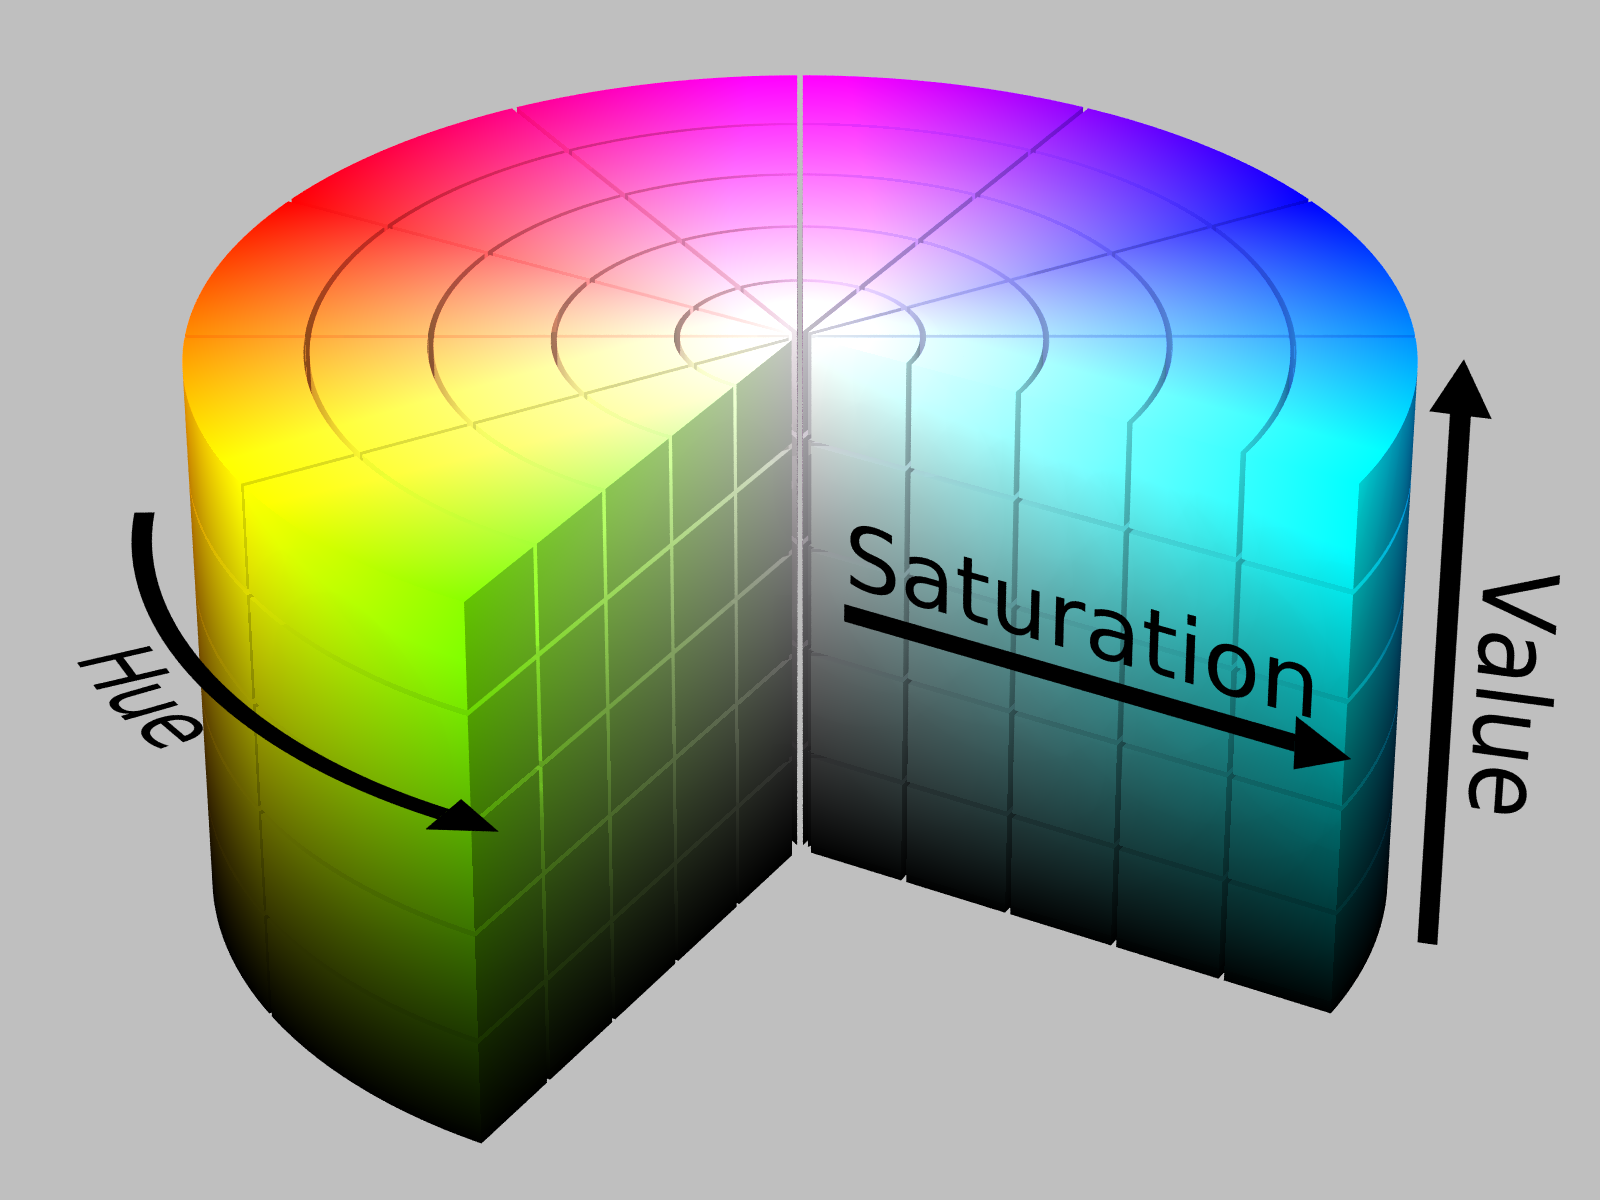
\includegraphics[width=0.3\textwidth]{Imagenes/hsv.png}
		\caption{Espacio de colores HSV representado como un cilindro.}
		\label{fig:hsv}
\end{figure}

Este espacio se puede representar como un cilindro, como se demuestra en la Figura (\ref{hsv}). Si bien la componente de value representa la oscuridad/luminosidad de un color, este modelo es incorrecto debido a que presenta uniformidades. Es por esto, que para obtener una verdadera representación de luminosidad se utiliza el espacio Lab.
El espacio de color L*a*b* de la comisión internacional en iluminación o CIE por sus siglas en francés es un espacio de color perceptualmente uniforme que representa a un color mediante tres parámetros: lightness, a y b, siendo lightness un modelo correctamente calculado e uniforme de la luminosidad de un color, y a y b las componentes de rojo/verde y amarillo/azul del color respectivamente\footnote{Imagen atribuida en \href{https://opentextbc.ca/graphicdesign/chapter/colour-science/}{https:\slash \slash opentextbc.ca\slash graphicdesign\slash chapter\slash colour-science\slash}}.
\begin{figure}[H]
		\centering
		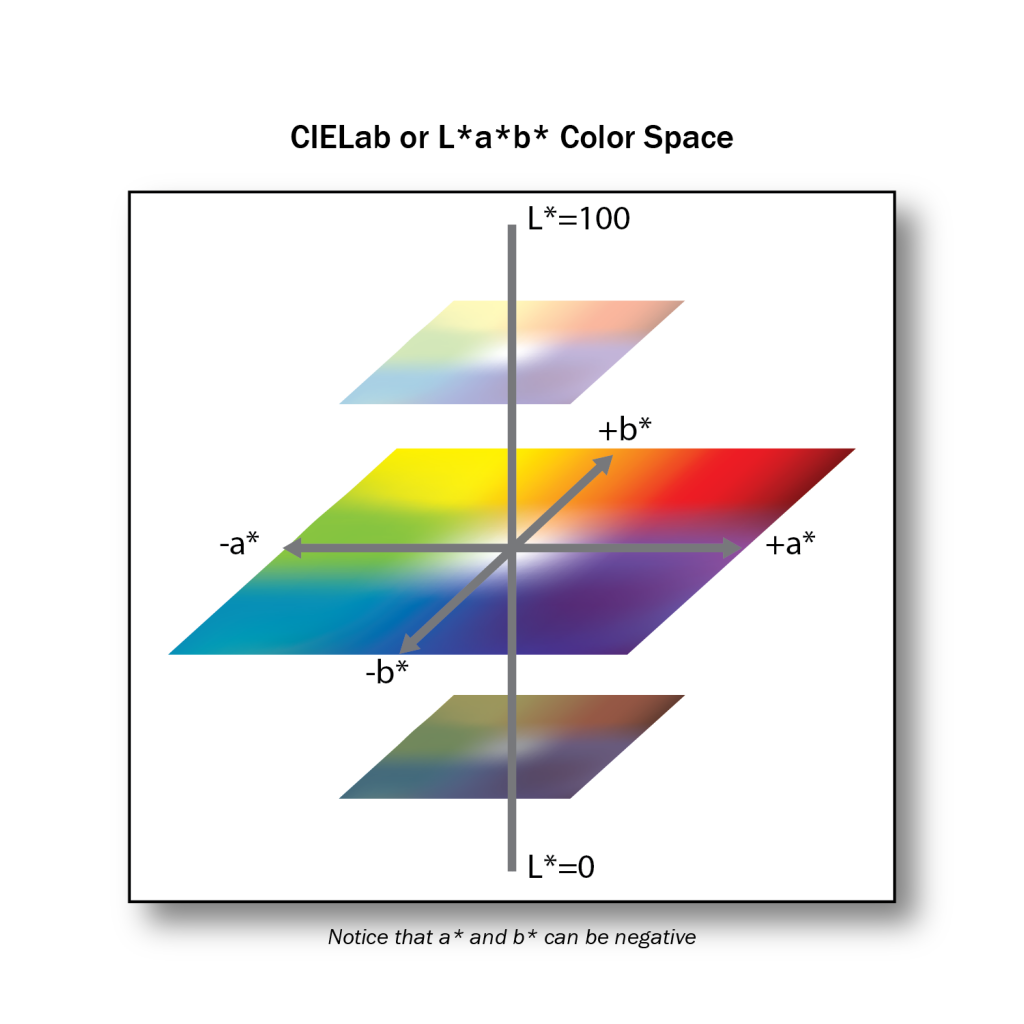
\includegraphics[width=0.3\textwidth]{Imagenes/lab.png}
		\caption{Espacio de colores CIE-Lab en el espacio cartesiano.}
		\label{fig:lab}
\end{figure}

